
%\fitter\ is a unique QCD fit platform that provides many options to the user to perform a quantitative assessment of impact level for a new data or new theoretical prediction. The quest on nailing down the uncertainties on PDFs have lead, on one hand, to highly precise measurements that are in need of careful handling of all provided sources of uncertainties, and on the other hand to numerous software packages that provide higher order calculations in QCD to match the precision of data.


When performing a QCD analysis to determine PDFs there are various assumptions and choices to be made concerning, for example, the functional form of the input parametrisation, the treatment of heavy quarks and their mass values, alternative theoretical calculations, alternative representations of the fit $\chi^2$ and for different ways of treating correlated systematic uncertainties.
%
 It is useful to discriminate or quantify the effect of a chosen ansatz within a common framework and 
\fitter is optimally designed for such tests.
%
The methodology employed by \fitter  relies on a flexible and modular
framework that allows independent integration of state-of-the-art techniques, either related to the inclusion of a new theoretical calculation, or of new approaches to treat data and their uncertainties. 

In this section we describe the available options for the fit methodology in \fitter.
%ranging from the functional form used to parametrise PDFs and the choice of the form of the $\chi^2$ function, to different methods to assess the experimental uncertainties on extracted PDFs.
%
%list various types of functional forms used to parametrise PDFs, different definitions for  $\chi^2$ evaluation in extracting the PDF parameters which account for correlated and uncorrelated sources of experimental (or theoretical) uncertainties available in \fitter. 
In addition, as an alternative approach to a complete QCD fit, the Bayesian reweighting
method, which is also available in \fitter, is described.
\subsection{Functional Forms for PDF Parametrisation}
The PDFs can be parametrised using several predefined
functional forms and flavour decompositions:
\paragraph{Standard Polynomials:} 
The standard polynomial form is the most commonly used. A polynomial functional form is used to parametrise the $x$-dependence of the PDFs, where index $j$ denotes each parametrised PDF flavour:
\begin{equation}
\centering
 xf_j(x) = A_j x^{B_j} (1-x)^{C_j} P_j(x).
\label{eqn:pdf_std}
\end{equation}
The parametrised PDFs are the valence distributions
$xu_v$ and $xd_v$, the gluon distribution $xg$, and the light sea quark distributions,
% as constrained by HERA data alone,
$x\bar{u}$, $x\bar{d}$,
% where $x\bar{U} = x\bar{u}$, 
$x\bar{s}$, at the starting scale, which is 
chosen below the charm mass threshold. 
The form of polynomials $P_j(x)$ can be varied.
% depend on the style and is defined as a steerable parameter. 
The form $(1 + \epsilon_j \sqrt{x} + D_j x + E_j x^2)$
is used for the HERAPDF \cite{h1zeus:2009wt} 
with additional constraints relating to the flavour decomposition of the 
light sea. This parametrisation is termed HERAPDF-style. The polynomial can also
be parametrised in the CTEQ-style, where $P_j(x)$ takes the form $e^{a_3x} (1 + e^{a_4} x + e^{a_5} x^2)$ and,
in contrast to  the HERAPDF-style, this is positive by construction.
QCD number and momentum sum rules are used to determine the normalisations $A$ for the valence and gluon
distributions, and the sum-rule integrals are solved analytically.
\paragraph{Bi-Log-Normal Distributions:} 
%A bi-log-normal distribution to parametrise the $x$ dependence of the PDFs is 
%also available in \fitter.
%parton distribution function of the proton.
This parametrisation is motivated by multi-particle statistics
%~\cite{hera-lhc:report2009}
and has the following functional form:
%\begin{center}
\begin{equation}
 xf_j(x)=a_j x^{p_j-b_j\log(x)}(1-x)^{q_j-d_j \log(1-x)}.
\label{eqn:bilog}
\end{equation}
%\end{center}
This function can be regarded as a generalisation of the standard polynomial form described above,
however, numerical integration of Eq.~\ref{eqn:bilog} is required in order to impose the QCD sum rules.
%In order to satisfy the QCD sum rules this parametric form requires numerical integration.
\paragraph{Chebyshev Polynomials:} 
A flexible parametrisation  based on the Chebyshev polynomials can be employed for the gluon and sea distributions.
Polynomials with argument $\log(x)$ are considered for better modelling the low-$x$ asymptotic behaviour of those PDFs. 
The polynomials are multiplied
by a factor of $(1-x)$ to ensure that they vanish as $x\to 1$. The resulting parametric form reads
\begin{eqnarray}
x g(x) &=& A_g \left(1-x\right) \sum_{i=0}^{N_g-1} A_{g_i} T_i \left(-\frac{\textstyle 2\log x - \log x_{\rm min} } {\textstyle \log x_{\rm min} } \right)\,, \label{eq:glu} \\
x S(x) &=& \left(1-x\right) \sum_{i=0}^{N_S-1} A_{S_i} T_i \left(-\frac{\textstyle 2\log x - \log x_{\rm min} } {\textstyle \log x_{\rm min} } \right)\,, \label{eq:sea} 
\end{eqnarray}
where $T_i$ are first-type Chebyshev polynomials of order $i$.
%The values of $N_{g,S}$ up to 15 are allowed, however, already
%starting from $N_{g,S}>5$ the fit quality is similar to the one based on
%the standard-polynomial parametrisation with a similar number of parameters.
The normalisation factor $A_g$ is derived from the momentum sum rule analytically.
Values of $N_{g,S}$ to $15$ are allowed, however the fit quality is already similar
to that of the standard-polynomial parametrisation from $N_{g,S} \ge 5$  and has a similar number of free parameters.
%
%where the sum runs over $i$ up to $N_{g,S}=15$ order Chebyshev polynomials of the first type $T_i$ for
%the gluon, $g$, and sea-quark, $S$, density, respectively. 
%The normalisation factor $A_g$ is defined from the momentum sum rule.
%%
%The advantages of this parametrisation are that the momentum sum rule can be evaluated analytically 
%and that for $N \ge 5$ the fit quality is already similar
%to the standard Regge-inspired parametrisation with a similar number of parameters.
%A study of the parametrisation uncertainty at low Bjorken $x \le 0.1$ for PDFs was presented 
%in~\cite{Chebyshev}. Figure~\ref{fig:cheb} shows the comparison of the 
%gluon density detemined from the HERA data  
%with the standard and the Chebyshev parametrisation.
%
%The low-$x$ uncertainties in the PDFs determined from the HERA data using different 
%parametrisatons were studied in Ref.~\cite{Chebyshev}.
Fig. \ref{fig:cheb} (taken from \cite{Chebyshev})
shows a comparison of the gluon distribution obtained with the parametrisation Eqs.~\ref{eq:glu}, \ref{eq:sea} to 
the standard-polynomial one, for $N_{g,S} = 9$.

%with a reduced parametrisation uncertainty. 
%An additional regularisation prior leads to a 
%significantly reduced uncertainty for $x \le 0.0005$.
\begin{figure}[!ht]
 \centering
%  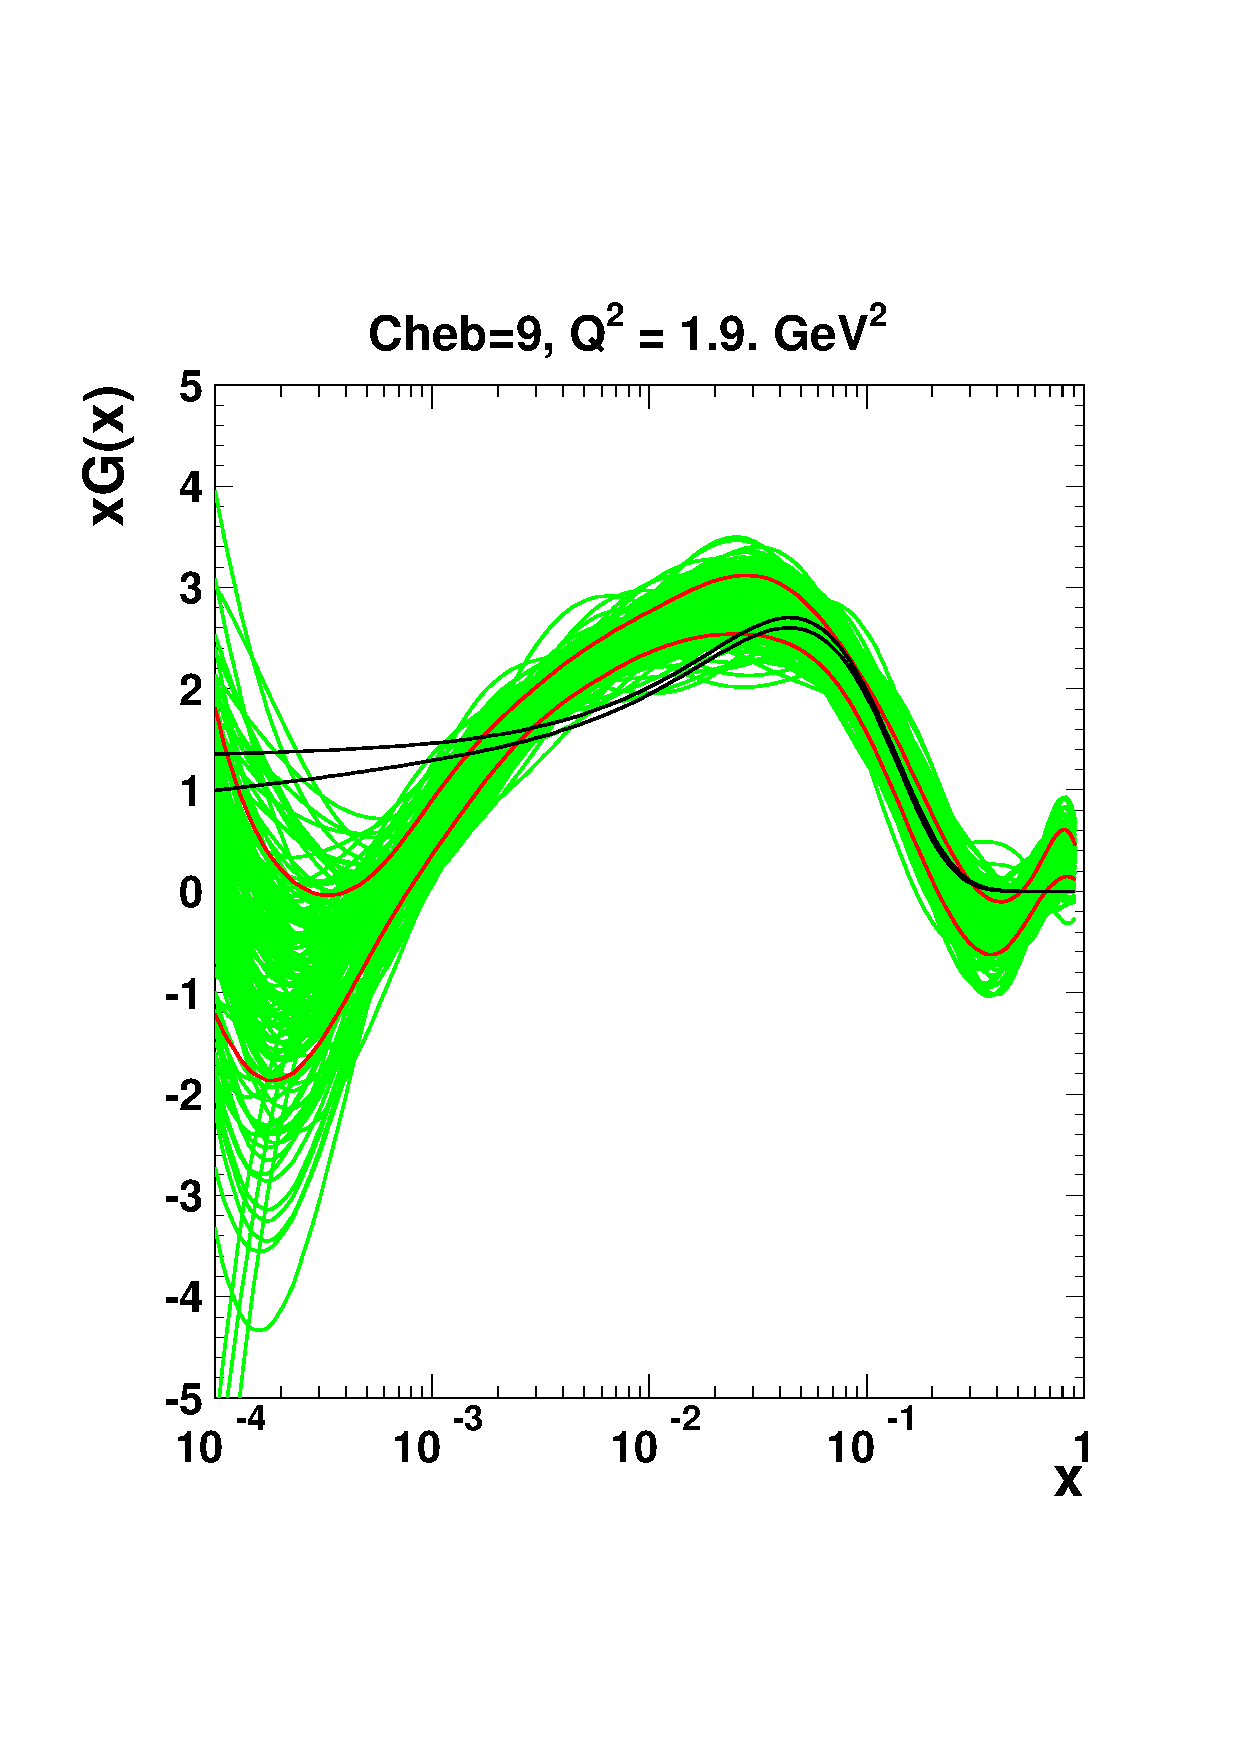
\includegraphics[width=5cm]{chebishev.pdf}
  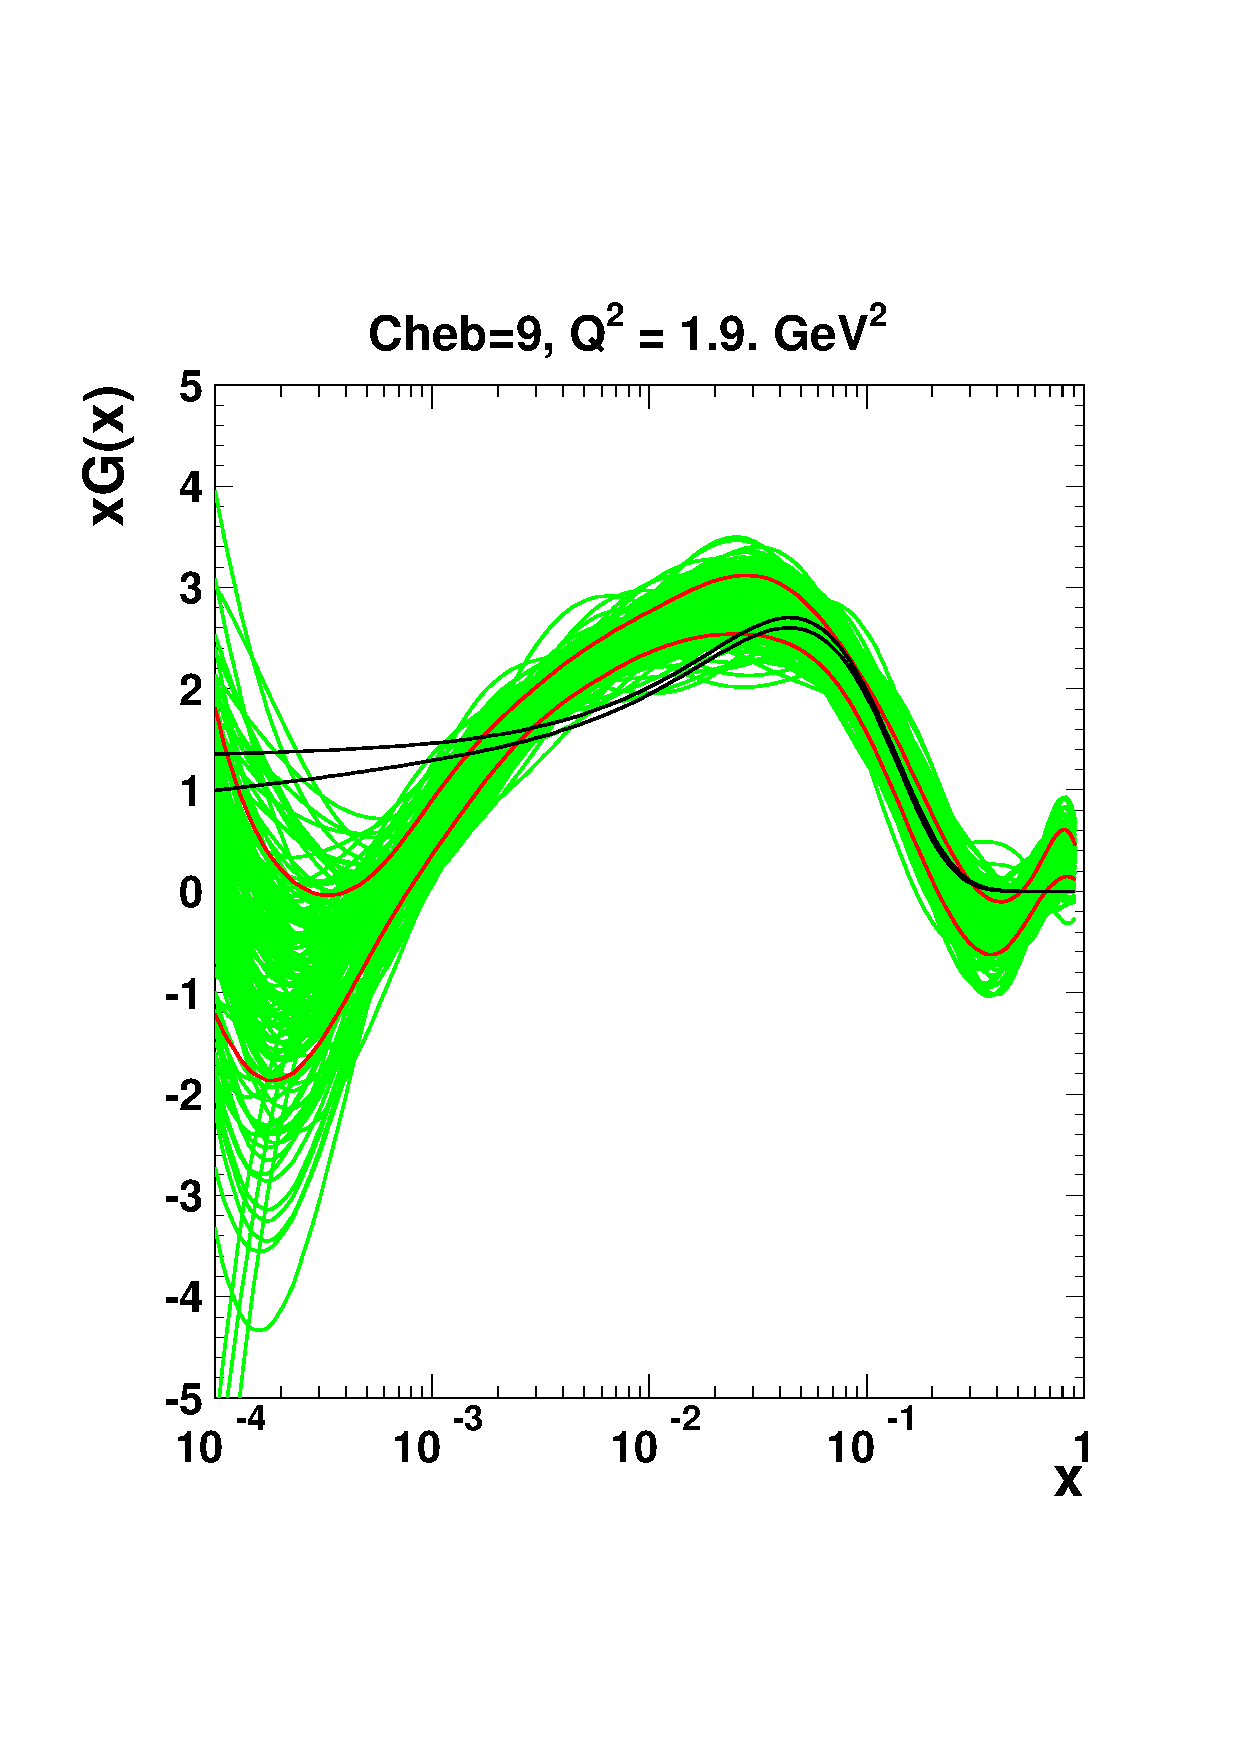
\includegraphics[trim=1cm 4cm 1cm 5cm, clip, width=6cm]{chebishev.pdf}
% \caption{Gluon PDF at the scale of $Q^2=1.9 \  \GeV^2$ for various values of the length-prior 
% weight $\alpha$ \cite{Chebyshev} using the Chebyshev parametrisation expanded to the 15th order.}
  \caption{The gluon density is shown at the starting scale $Q^2=1.9$ GeV$^2$. The black lines correspond to the uncertainty band of the gluon distribution using a standard parametrisation and it is compared to the case of the Chebyshev parametrisation \cite{Chebyshev}. The uncertainty band for the latter case is estimated using the Monte Carlo technique (see Sec. \ref{sec:experimentalerrors}) with the green lines denoting fits to data replica.  Red lines indicate the standard deviation about the mean value of these replicas.}
 \label{fig:cheb}
\end{figure}

%
\paragraph{External PDFs:} \rm 
 \fitter also provides the possibility to access external PDF sets, which can be used to compute 
theoretical predictions for the cross sections for all the processes available in \fitter. 
This is possible via an interface to \lhapdf~\cite{lhapdf,lhapdfweb} providing access to the 
global PDF sets.
%available at different orders.
%\fitter also allows one to evolve PDFs from \lhapdf with \qcdnum using the corresponding grids as a starting scale.
\fitter also allows one to evolve PDFs from \lhapdf using \qcdnum.
%using the corresponding grids as a starting scale.
%locally through the \fitter or taken as provided by the \lhapdf grids. 
Fig. \ref{fig:pdfs} illustrates a comparison of various gluon PDFs accessed from \lhapdf as produced with the drawing 
tools available in \fitter.
%\end{description}
%
\begin{figure}[!ht]
   \centering
   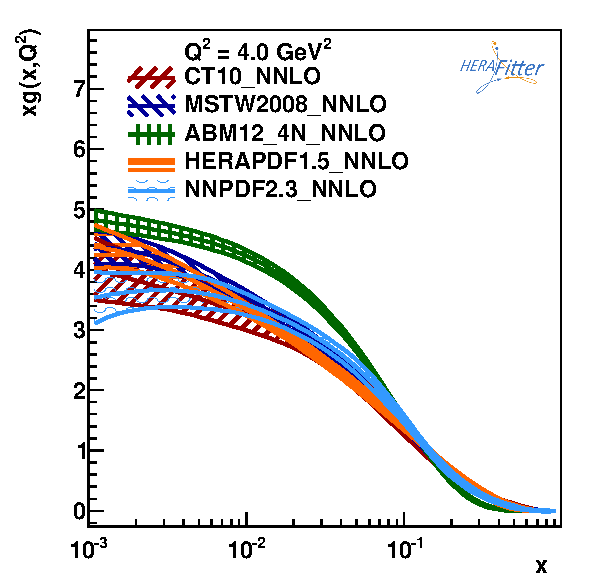
\includegraphics[width=8cm]{pdfs.pdf}
   \caption{The gluon PDF as extracted by various groups at the scale of $Q^2=4 \ \GeV^2$, plotted using the drawing tools from \fitter.} 
 \label{fig:pdfs}
\end{figure}
%
% --- ascii:
% \subsection{Representation of \texorpdfstring{$\chi^2$}{chi squared}}
% --- utf8:
\subsection{Representation of \texorpdfstring{$\chi^2$}{χ²}}
% \subsection{Representation of $\chi^2$}
\label{sec:chi2representation}

The PDF parameters are determined in \fitter by minimisation of a
$\chi^2$ function taking into account correlated and uncorrelated measurement uncertainties.
%The PDF parameters are extracted in a $\chi^2$ minimisation process.
%The construction of the $\chi^2$  accounts for the experimental uncertainties.
There are various forms of $\chi^2$, 
e.g. using a covariance matrix or providing nuisance parameters to encode the dependence of 
each correlated systematic uncertainty for each measured data point.
%, different scaling options, etc. 
%In addition, there are various methods to deal with correlated systematic (or statistical) uncertainties. 
The options available in \fitter are the following:
\begin{description}
\item \it {Covariance Matrix Representation:} \rm
For a data point $\mu_i$ with a corresponding theory prediction $m_i$, 
the $\chi^2$ function 
can be expressed in the following form:
%
\begin{eqnarray}
\chi^2 (m)& = & \sum_{i,k}(m_i-\mu_i)C^{-1}_{ik}(m_k-\mu_k),
\end{eqnarray}
where the experimental uncertainties are given as a covariance matrix $C_{ik}$ for measurements in bins $i$ and $k$.
%The $\chi^2$ function depends on the theory parameters $m^i$ 
%(denoted as the vector $\boldsymbol{m}$).
The covariance matrix $C_{ik}$ is given by a sum of statistical, uncorrelated and correlated systematic contributions: 
\begin{eqnarray}
C_{ik}& = & C^{stat}_{ik}+C^{uncor}_{ik}+C^{sys}_{ik}.
\end{eqnarray}
Using this representation one cannot distinguish the effect of each source of systematic uncertainty. 
\item \it{Nuisance Parameter Representation:} \rm
In this case, the $\chi^2$ is expressed as
\label{sec:nuisance_representation}
%\begin{eqnarray} 
%    \chi^2\left(\boldsymbol{m},\boldsymbol{b}\right) &= &  
% \sum_i \frac{\left[m^i - \sum_j \gamma^i_j m^i b_j  - {\mu^i} \right]^2}
%{ \textstyle \delta^2_{i,{\rm stat}}\mu^i \left(m^i -  \sum_j \gamma^i_j m^i b_j\right)
%  + \left(\delta_{i,{\rm uncor}}\,  m^i\right)^2} \nonumber \\
%  &+& \sum_j b^2_j.
%\label{eq:aven}
%\end{eqnarray}
%{ \small
%\begin{equation} 
%    \chi^2\left(\boldsymbol{m},\boldsymbol{b}\right) =   
% \sum_i \frac{\left[m^i - \sum_j \gamma^i_j m^i b_j  - {\mu^i} \right]^2}
%{ \textstyle \delta^2_{i,{\rm stat}}\mu^i \left(m^i -  \sum_j \gamma^i_j m^i b_j\right)
%  + \left(\delta_{i,{\rm uncor}}\,  m^i\right)^2}+ \sum_j b^2_j.
%\label{eq:aven}
%\end{equation}}
\begin{equation} 
    \chi^2\left(\boldsymbol{m},\boldsymbol{b}\right) =   
 \sum_i \frac{\left[ {\mu_i} - m_i \left( 1 - \sum_j \gamma^i_j b_j \right) \right]^2}
{ \textstyle \delta^2_{i,{\rm unc}}m_i^2 + \delta^2_{i,{\rm stat}}\, {\mu_i} m_i \left(1 - \sum_j \gamma^i_j b_j\right) }
  + \sum_j b^2_j,
\label{eq:aven}
\end{equation}
%
where, $\delta_{i,\rm stat}$ and $\delta_{i,\rm unc}$ are 
relative statistical and uncorrelated systematic uncertainties
of the measurement $i$.
%where, ${\mu_i}$ is the central value of the measurement $i$ 
% ${\mu_i}$ is the central value of the measurement $i$ 
%with its relative statistical $\delta_{i,\rm stat}$ 
%and relative uncorrelated systematic uncertainty $\delta_{i,\rm unc}$.
Further, $\gamma^i_j$ quantifies the sensitivity of the
measurement to the correlated systematic source $j$. 
The function $\chi^2$ depends on
 the set of systematic nuisance parameters $b_j$.
This definition of the $\chi^2$ function assumes that
systematic uncertainties are proportional to the central prediction values
(multiplicative uncertainties, $m_i(1-\sum_j\gamma_j^ib_j)$), whereas the statistical uncertainties scale 
with the square root of the expected number of events. 
However, additive treatment of uncertainties is also possible in \fitter.
% ($m_i+\sum_j\Gamma_j^ib_j$, where $\Gamma_j^i$ is correlated systematic uncertainty)


During the $\chi^2$ minimisation, the nuisance parameters $b_j$ and the PDFs are determined, such that the effect of different sources of systematic uncertainties can be distinguished.
%The nuisance parameters $b_j$ as well as the PDF parameters are free parameters of the fit. 
%The fit determines the best PDF parameters to
%the data taking into account correlated systematic shifts of the data. 
\item  \it{Mixed Form Representation:} \rm
In some cases, the statistical and systematic uncertainties of experimental data are provided in different forms.    
%It can happen that various parts of the systematic and statistical uncertainties are stored in different forms. 
For example, the correlated experimental systematic uncertainties are available as nuisance parameters,
but the bin-to-bin statistical correlations are given in the form of a covariance matrix.
%A situation can be envisaged when the correlated systematic experimental uncertainties are provided as nuisance parameters, but the statistical bin-to-bin correlations are given in the form of a covariance matrix. 
\fitter\ offers the possibility to include such mixed forms of information. 
%information, when provided, as well as any other mixed 
%for treating statistical, uncorrelated and correlated systematic uncertainties. 
%In the case of off-diagonal statistical uncertainties, the $\chi^2$ function
%\begin{equation} 
%\begin{eqnarray} 
% \label{eq:chi2gen}
%    \chi^2(\boldsymbol{m},\boldsymbol{b})& = & \sum_{ij} 
%         \left ( m^i - \sum_l \gamma^i_l(m^i)b_l - \mu^i \right)  C^{-1}_{{\rm stat.}~ij}(m^i,m^j) \nonumber \\  
%    && \left(  m^j - \sum_l \gamma^j_l(m^j)b_l - \mu^j \right) +  \sum_l b^2_l.
%\end{eqnarray}
%\end{equation}
%Here the scaling properties of the correlated systematic uncertainties 
%$\Gamma^i_j$ and
%of the covariance matrix $C_{{\rm stat.}~ij}$ are expressed as a dependence
%on $m_i$ and the dependence of $\delta_{\rm stat}$ on $b_j$ is ignored.
\end{description}
Any source of measured systematic uncertainty can be treated as additive or multiplicative, as described above. 
The statistical uncertainties can be included as additive or following the Poisson statistics. Minimisation
with respect to nuisance parameters is performed analytically, however, for more 
detailed studies of correlations individual nuisance parameters can be included into 
the \minuit minimisation.



\subsection{Treatment of the Experimental Uncertainties}
\label{sec:experimentalerrors}


Three distinct methods for propagating experimental uncertainties to PDFs are implemented in \fitter and reviewed here:
%\fitter\ provides three methods for assessing the experimental uncertainties on PDFs: 
the Hessian, Offset, and Monte Carlo method.
%Figure \ref{fig:error} illustrates the difference between the Hessian and Monte-Carlo methods both of which can be applied and plotted with \fitter.
%\begin{figure}[!ht]
%   \centering
%   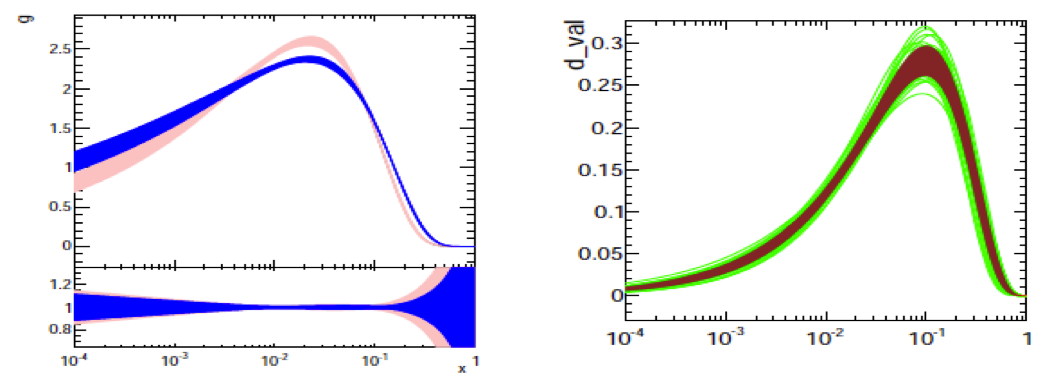
\includegraphics[width=8cm]{error.pdf}
%   \put (-206, 68) {Hessian}
%   \put (-86, 68) {Monte Carlo}
%   \caption{Differences in the experimental uncertainties on the gluon (left) and d-valence quark (right) densities extracted 
%       through different methods in \fitter: Hessian(left) versus Monte Carlo (right).} 
% \label{fig:error}
%\end{figure}
\begin{description}
\item \it{Hessian (Eigenvector) method:} \rm
The PDF uncertainties reflecting the data experimental uncertainties are estimated by 
examining the shape of the $\chi^2$ function in the neighbourhood of the minimum \cite{Pumplin:2001ct}.
%The technique developed in~\cite{Pumplin:2001ct} presents an estimate of PDF uncertainties 
%reflecting the experimental precision of data used in the QCD fit by examining the behavior 
%of $\chi^2$ in the neighborhood of the minimum. 
Following the approach of Ref. \cite{Pumplin:2001ct}, the Hessian matrix is defined by the second 
derivatives of $\chi^2$ on the fitted PDF parameters. The matrix is diagonalised and the 
Hessian eigenvectors are computed. 
Due to orthogonality these vectors correspond to independent sources of
uncertainty in the obtained PDFs.
\\
%
%This is known as the Hessian or error matrix method. 
%The Hessian matrix is built by the second derivatives of $\chi^2$ at the minimum. 
%The Hessian matrix is diagonalised through an iterative procedure and its PDF eigenvectors
%are obtained, which correspond to the orthogonal sources of uncertainties on the obtained PDF.

\item \it{Offset  method:} \rm
The Offset method \cite{Botje:2001fx} uses
%Another method to propagate the correlated systematic experimental uncertainties from 
%the measurements to PDFs \cite{Botje:2001fx} is Offset method.
%, which has the practical advantage that it does not require the inversion of a large measurement covariance matrix.
%
the $\chi^2$ function for the central fit, but only
uncorrelated uncertainties are taken into account. 
The goodness of the fit can no longer be judged from the $\chi^2$ since correlated uncertainties are ignored. 
The correlated uncertainties are propagated into the PDF uncertainties by performing variants 
of the fit with the experimental data varied by $\pm 1 \sigma$ from the central value  
for each systematic source.
The resulting deviations of the PDF parameters from the ones obtained in the central 
fit are statistically independent, and they can be combined in quadrature to derive a total 
PDF systematic uncertainty.
%
%Instead, the correlated systematic uncertainties of the measurement are used to estimate 
%the errors on the PDF parameters as follows.
%The cross section is varied by $\pm 1 \sigma$ from the central value 
%for each systematic source and the fit is performed. 
%After this has been done for all sources, the 
%resulting deviations of each of these fits from the central PDF parameters are added in quadrature. 

The uncertainties estimated by the offset method are generally larger than 
those from the Hessian method.
\\
%as the offset method does not use the information on correlated systematic uncertainties 
%in the central fit.

\item \it{Monte Carlo method:} \rm
The Monte Carlo (MC) technique \cite{Giele:1998gw, mcmethod2} can also be used to determine PDF uncertainties.
The uncertainties are estimated using pseudo-data replicas (typically $>100$) 
randomly generated from the measurement central values and their systematic and statistical uncertainties 
taking into account all point-to-point correlations.
%
The QCD fit is performed for each replica and the PDF central values and their 
experimental uncertainties are estimated from the distribution of the PDF parameters obtained in these fits, by taking 
the mean values and standard deviations over the replicas.
%
%The preparation of the data is repeated for large $N$ ($>100$ times) and for each of these replicas a QCD fit is performed. 
%The PDF central values and experimental uncertainties are estimated using the mean values 
%and standard deviations over the replicas.

%The MC method represents one of the main concepts of the NNPDF group.
The MC method has been checked against the standard error estimation of the PDF uncertainties obtained by the Hessian method. 
A good agreement was found between the methods provided that Gaussian distributions of statistical and systematic uncertainties are assumed in the MC 
approach~\cite{hera-lhc:report2009}.
%when employing for the MC approach the assumption that uncertainties 
%(statistical and systematic) follow Gaussian distribution~\cite{hera-lhc:report2009}. 
A comparison is illustrated in Fig.~\ref{fig:mchessian}. 
Similar findings were reported by the MSTW global analysis~\cite{Watt:2012tq}. 
\begin{figure}[!ht]
 \centering
%  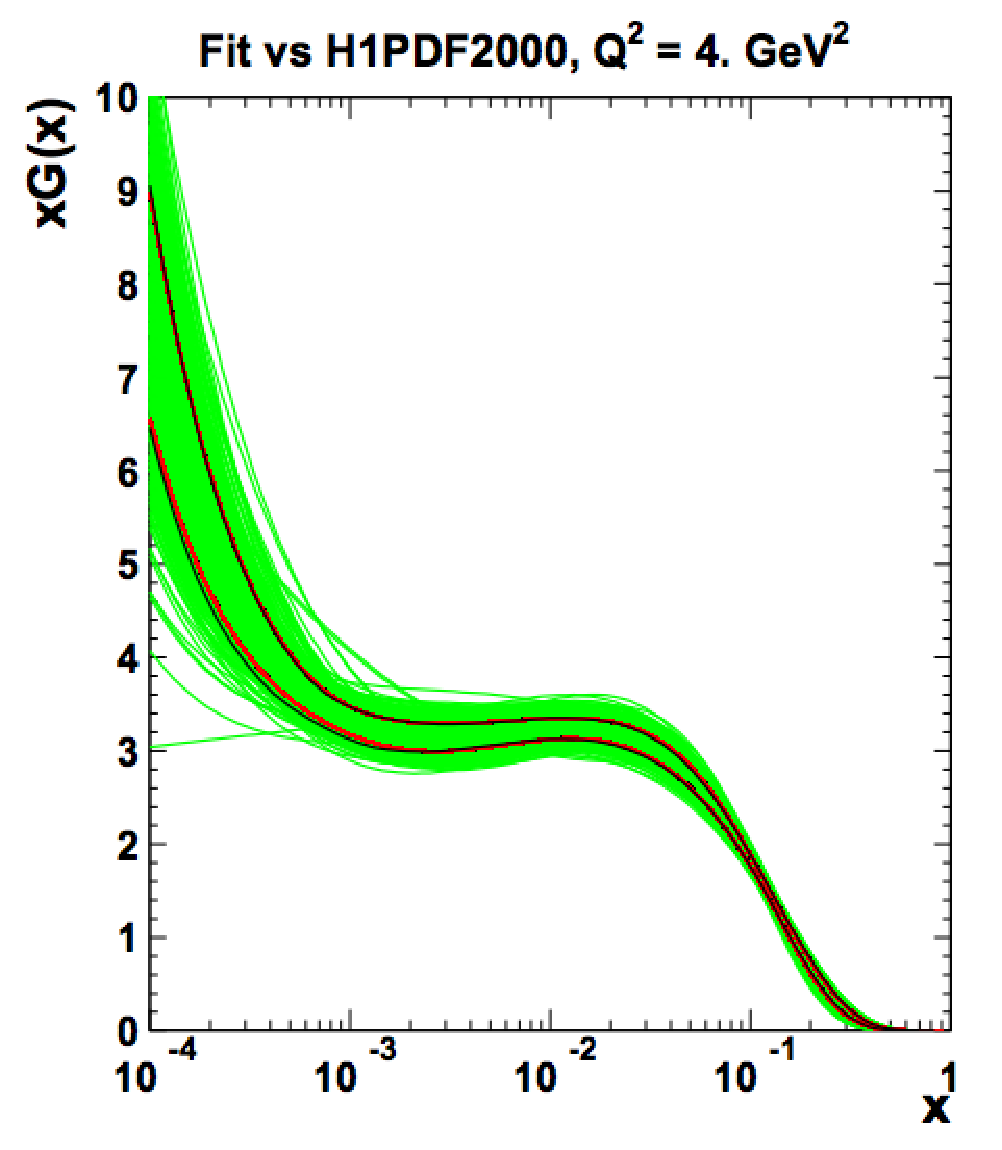
\includegraphics[width=7cm,height=7cm]{mchessian.pdf}
  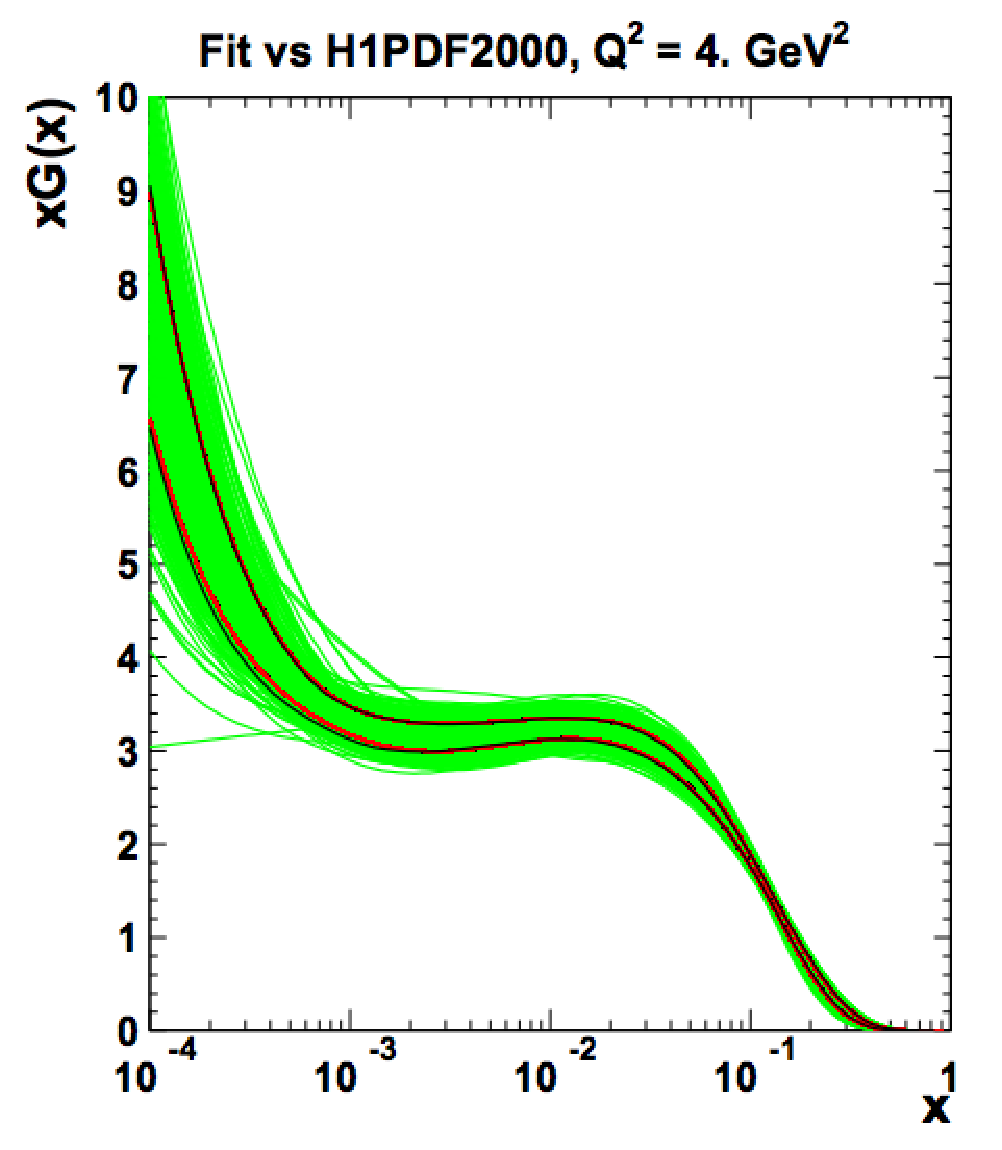
\includegraphics[trim=1cm 4cm 1cm 5cm, clip, width=6.3cm]{mchessian.pdf}
  \caption{Comparison between the standard error calculations as employed by the Hessian approach (black lines) 
           and the MC approach (with more than 100 replicas) assuming Gaussian distribution for uncertainty 
           distributions, shown here for each replica 
          (green lines) together with the evaluated standard deviation (red lines) \cite{hera-lhc:report2009}.
          The black and red lines in the figure are superimposed because agreement of the methods is so good that it is hard to distinguish them.}
  \label{fig:mchessian}        
\end{figure}
%

Since the MC method requires large number of replicas, the eigenvector representation 
is a more convenient way to store the PDF uncertainties.
It is possible to transform MC to eigenvector
representation as shown by \cite{Gao:2013bia}. Tools to perform this transformation are provided with \fitter and were 
recently employed for the representation of correlated sets of PDFs at different perturbative orders \cite{hfcorrpaper}.
%
\end{description}
%
The nuisance parameter representation of $\chi^2$ in Eq.~\ref{eq:aven} is derived assuming 
symmetric experimental errors, however, the published systematic uncertainties are 
often asymmetric.
%Generally, the experimental uncertainties using nuisance parameters are 
%symmetrised when QCD fits 
%are performed, however often the provided uncertainties are rather asymmetric.
\fitter provides the possibility to use asymmetric systematic uncertainties.
The implementation relies on the assumption that 
asymmetric uncertainties can be described by a parabolic function.
The nuisance parameter in Eq.~\ref{eq:aven} is modified as follows
\begin{equation}
  \gamma^i_{j} \to \omega^i_{j}b_j + \gamma^i_{j},
\end{equation}
where the coefficients $\omega^i_{j}$, $\gamma^i_{j}$ are defined  
from the maximum and minimum shifts of the cross sections due to a  variation of the systematic uncertainty $j$, 
$S_{ij}^{\pm}$,
\begin{equation}
  \omega^i_{j}=\frac{1}{2}\left(S_{ij}^{+}+S_{ij}^{-}\right), \\
  \gamma^i_{j}=\frac{1}{2}\left(S_{ij}^{+}-S_{ij}^{-}\right). 
\end{equation}
%For this case the definition of the $\chi^2$ from Eq.~\ref{eq:aven} is extended with the parabolic approximation 
%for asymmetric uncertainties, such that the expected cross section is adjusted to be
%\begin{equation}
%  m_i(1-\sum_j \gamma^i_{j} b_j) \to 
%m_i\left(1-\sum_j b_j(\omega^i_{j}b_j + \gamma^i_{j})\right).
%\end{equation}
%%The minimisation is performed using fixed number of iterations (typically ten), with rapid convergence.



\subsection{Treatment of the Theoretical Input Parameters}
\label{sec:theoryerr}

The results of a QCD fit depend not only on the input data but also on the 
input parameters used in the theoretical calculations. Nowadays, PDF groups 
address the impact of the choices of theoretical parameters by providing
alternative PDFs with different choices of the mass of the charm quarks, $m_c$, 
mass of the bottom quarks, $m_b$, and the value of $\asmz$. 
Other important aspects are the choice of the functional form for the PDFs at the 
starting scale and the value of the starting scale itself. \fitter provides the
possibility of different user choices of all these inputs.% to the theory.
%a platform in which such choices can readily be varied within a common framework.

\subsection{Bayesian Reweighting Techniques}

As an alternative to performing a full QCD fit, \fitter allows the user to assess the impact of including new
data in an existing fit using the Bayesian Reweighting technique. The method
provides a fast estimate of the impact of new data on PDFs. 
Bayesian Reweighting was first proposed for PDF sets delivered in the form of MC replicas by~\cite{Giele:1998gw} 
and further developed by the NNPDF Collaboration~\cite{Ball:2011gg,Ball:2010gb}. 
More recently, a method to perform Bayesian Reweighting studies starting from PDF fits for which uncertainties
are provided in the eigenvector representation has been also developed~\cite{Watt:2012tq}. The latter is 
based on generating replica sets by introducing Gaussian fluctuations on the central PDF set with a variance 
determined by the PDF uncertainty given by the eigenvectors. Both reweighting methods are implemented in \fitter.
Note that the precise form of the weights used by both methods has recently been questioned \cite{Sato:2013ika,Paukkunen:2014zia}.

The Bayesian Reweighting technique relies on the fact that MC replicas of a PDF set give 
a representation of the probability distribution in the space of PDFs. In particular, the PDFs are represented 
as ensembles of $N_{\rm rep}$ equiprobable ({\em i.e.} having weights equal to unity) replicas, $\{f\}$. 
The central value for a given observable, $\mathcal{O}(\{f\})$, is computed as the average of the 
predictions obtained from the ensemble as
\begin{equation}
\langle\mathcal{O}(\{f\})\rangle =  \frac{1}{N_{\mathrm{rep}}} \sum_{k=1}^{N_{\mathrm{rep}}} \mathcal{O}(f^{k}),
\end{equation}
and the uncertainty as the standard deviation of the sample.

Upon inclusion of new data the prior probability distribution, given by the original PDF set, is modified according
to Bayes Theorem such that the weight of each replica, $w_k$, is updated according to
\begin{equation}
 w_k = \frac{(\chi^2_k)^{\frac{1}{2} (N_{\mathrm{data}}-1) } e^{-\frac{1}{2}\chi^2_k}}
          { \frac{1}{N_{\mathrm{rep}}} \sum^{N_{\mathrm{rep}}}_{k=1}(\chi^2_k)^{\frac{1}{2}(N_{\mathrm{data}}-1)} e^{-\frac{1}{2}\chi^2_k}  },
\end{equation}
where $N_{\mathrm{data}}$ is the number of new data points, $k$ denotes the specific replica for which the 
weight is calculated and $\chi^2_k$ is the $\chi^2$ of the new data obtained using the $k$-th PDF replica.
%{\small
%\begin{equation}
%% \chi^2 (y,\mathrm{PDF}_k) = \sum_{i,j=1}^{N_{\mathrm{data}}} (y_i - y_i(\mathrm{PDF}_k)) \sigma^{-1}_{ij} (y_j-y_j(\mathrm{PDF}_k))\,. 
% \chi^2 (m,\mathrm{PDF}_k) = \sum_{i,j=1}^{N_{\mathrm{data}}} \left( m_i - m_i(\mathrm{PDF}_k)\right) \sigma^{-1}_{ij} (m_j-m_j\left(\mathrm{PDF}_k)\right)\,. 
%\end{equation}
%}
Given a PDF set and a corresponding set of weights, which describes the impact of the
inclusion of new data, the prediction for a given observable after inclusion of the new data can be computed as the {\em weighted} average,
\begin{equation}
\langle\mathcal{O}(\{f\})\rangle =  \frac{1}{N_{\mathrm{rep}}} \sum_{k=1}^{N_{\mathrm{rep}}} w_k \mathcal{O}(f^{k}).
\end{equation}

To simplify the use of a reweighted set, an unweighted set ({\em i.e.} a set of equiprobable replicas which incorporates 
the information contained in the weights) is generated according to the unweighting procedure described in~\cite{Ball:2011gg}. 
The number of effective replicas of a reweighted set is measured by its Shannon 
Entropy~\cite{Ball:2010gb}
\begin{equation}
\label{eq:shannon}
N_\mathrm{eff}\equiv 
\exp\left\{\frac{1}{N_\mathrm{rep}}\sum_{k=1}^{N_\mathrm{rep}}w_k\ln(N_\mathrm{rep}/w_k)\right\}\,,
\end{equation}
which corresponds to the size of a refitted equiprobable replica set containing the same amount of information. 
This number of effective replicas, $N_\mathrm{eff}$, gives an indicative measure of the optimal size of an 
unweighted replica set produced with the reweighting/unweighting procedure. No extra information is 
gained by producing a final unweighted set that has a number of replicas (significantly) larger than 
$N_\mathrm{eff}$.  If $N_\mathrm{eff}$ is much smaller than the original number of replicas the new data have great impact, however, it is unreliable to use the new reweighted set. In this case, instead, a full refit should be performed.

%On the one hand there is no reason in generating a final unweighted set that has a number of replicas
%(significantly) larger than $N_\mathrm{eff}$ as no extra information is gained. On the other hand it is
%advisable to start from a prior PDF set which has as many replicas as possible in order to have a more
%accurate posterior set at the end of the reweighting procedure.




